\pagenumbering{gobble}

\section*{Backup}

\begin{frame}
    \frametitle{}
    \centering
    \huge
    \alert{$>>>$ BACKUP}

\end{frame}

{
\begin{frame}
    \frametitle{Model Architecture}
    \begin{columns}
        \begin{column}{0.48\textwidth}
            \begin{figure}[h]
                \centering
                \resizebox{0.48\textwidth}{!}{%
            \begin{circuitikz}
            \tikzstyle{every node}=[font=\footnotesize]
            \draw [](6.25,15.5) to[short] (17.5,15.5);
            \draw (6.25,15.5) to[short] (17.5,15.5);
            \draw [](7.5,10.5) to[short] (16.25,10.5);
            \draw [short] (6.25,15.5) -- (7.5,10.5);
            \draw [short] (16.25,10.5) -- (17.5,15.5);
            \draw [](6.25,-8.25) to[short] (17.5,-8.25);
            \draw (6.25,15.5) to[short] (17.5,15.5);
            \draw [](7.5,-3.25) to[short] (16.25,-3.25);
            \draw [short] (16.25,-3.25) -- (17.5,-8.25);
            \draw [short] (6.25,-8.25) -- (7.5,-3.25);
            \node [font=\LARGE] at (11.75,13) {Encoder};
            \node [font=\LARGE] at (11.75,-5.75) {Decoder};
            \node [font=\normalsize, color=white] at (8.75,9) {Latent space};
            \draw [ color=white, short] (9.5,1.75) -- (9.5,0.5);
            \draw [ color=white, short] (9.5,1.75) -- (12,3);
            \draw [ color=white, short] (12,3) -- (12,-0.75);
            \draw [ color=white, short] (9.5,0.5) -- (12,-0.75);
            \node [font=\small] at (10.75,1.25) {Generator};
            \draw [ color=white ] (14.5,8.5) rectangle (15.75,8.25);
            \draw [ color=white ] (14.5,8.25) rectangle (15.75,8);
            \draw [ color=white ] (14.5,8) rectangle (15.75,7.75);
            \draw [ color=white ] (14.5,7.75) rectangle (15.75,7.5);
            \draw [ color=white ] (14.5,8.75) rectangle (15.75,8.5);
            \node [font=\small, color=white] at (15.25,7.25) {encoded heart beats};
            \draw [ color=white ] (14.5,1.75) rectangle (15.75,1.5);
            \draw [ color=white ] (14,1.5) rectangle (15.5,1.25);
            \draw [ color=white ] (14.5,1.25) rectangle (16,1);
            \draw [ color=white ] (14.25,1) rectangle (16.25,0.75);
            \draw [ color=white ] (14.75,0.75) rectangle (15.5,0.5);
            \node [font=\small, color=white] at (15.25,0.25) {Generated encodings};
            \draw [ color=white, ->, >=Stealth] (12,1.25) -- (13.75,1.25);
            \draw [color=white,](15,4.25) to[short, -*] (15,4.25);
            \node [font=\small] at (12.75,4.5) {MMD};
            \draw [ color=white, dashed] (15,4.25) -- (10.5,4.25);
            \draw [ color=white, ->, >=Stealth, dashed] (10.5,4.25) -- (10.5,2.5);
            \draw [ color=white , dashed] (7.75,1) circle (0.75cm);
            \node [font=\small, color=white] at (7.75,1) {Noise};
            \draw [ color=white, ->, >=Stealth] (8.5,1) -- (9.5,1);
            \draw [ color=white , dashed] (12,18.25) ellipse (7.75cm and 1cm);
            \node [font=\large] at (11.75,18.25) {Original heartbeats};
            \draw [->, >=Stealth] (12,17) .. controls (12,16.75) and (12,16.5) .. (12,15.75) ;
            \draw [ color=white , dashed] (11.75,-11) ellipse (7.75cm and 1cm);
            \draw [->, >=Stealth] (11.5,-8.5) -- (11.5,-9.75);
            \node [font=\large] at (11.5,-11) {Generated heartbeats};
            \draw [ color=white ] (15,5.75) circle (0.75cm);
            \node [font=\footnotesize] at (15,5.75) {DP noise};
            \draw [ color=white, ](15,7) to[short] (15,6.5);
            \draw [ color=white, ](15,5.0) to[short] (15,4.25);
            \draw [ color=white, dashed](15,1.75) to[short] (15,4.25);
            \draw [ color=white , dashed] (6.25,9.25) rectangle  (17.5,-2);
            \end{circuitikz}
            }%
            \caption{AE-(dp)MERF architecture}
            \end{figure}
        \end{column}
        
        \begin{column}{0.48\textwidth}
            \begin{figure}[h]
                \centering
                \resizebox{0.55\textwidth}{!}{%
                \begin{circuitikz}
                \tikzstyle{every node}=[font=\normalsize]
                \draw [](6.25,15.5) to[short] (17.5,15.5);
                \draw (6.25,15.5) to[short] (17.5,15.5);
                \draw [](7.5,10.5) to[short] (16.25,10.5);
                \draw [short] (6.25,15.5) -- (7.5,10.5);
                \draw [short] (16.25,10.5) -- (17.5,15.5);
                \draw [](6.25,-8.25) to[short] (17.5,-8.25);
                \draw (6.25,15.5) to[short] (17.5,15.5);
                \draw [](7.5,-3.25) to[short] (16.25,-3.25);
                \draw [short] (16.25,-3.25) -- (17.5,-8.25);
                \draw [short] (6.25,-8.25) -- (7.5,-3.25);
                \node [font=\LARGE] at (11.75,13) {Encoder};
                \node [font=\LARGE] at (9,-6) {Decoder};
                \node [font=\normalsize, color=white] at (6,8.75) {Latent space};
                \draw [ color=white, short] (6.75,1.5) -- (6.75,0.25);
                \draw [ color=white, short] (6.75,1.5) -- (9.25,2.75);
                \draw [ color=white, short] (9.25,2.75) -- (9.25,-1);
                \draw [ color=white, short] (6.75,0.25) -- (9.25,-1);
                \node [font=\small] at (8,1) {Generator};
                \draw [ color=white ] (11.75,8.25) rectangle (13,8);
                \draw [ color=white ] (11.75,8) rectangle (13,7.75);
                \draw [ color=white ] (11.75,7.75) rectangle (13,7.5);
                \draw [ color=white ] (11.75,7.5) rectangle (13,7.25);
                \draw [ color=white ] (11.75,8.5) rectangle (13,8.25);
                \node [font=\small, color=white] at (12.5,7) {encoded heart beats};
                \draw [ color=white ] (11.75,1.5) rectangle (13,1.25);
                \draw [ color=white ] (11.25,1.25) rectangle (12.75,1);
                \draw [ color=white ] (11.75,1) rectangle (13.25,0.75);
                \draw [ color=white ] (11.5,0.75) rectangle (13.5,0.5);
                \draw [ color=white ] (12,0.5) rectangle (12.75,0.25);
                \node [font=\small, color=white] at (12.5,0) {Generated encodings};
                \draw [ color=white, ->, >=Stealth] (9.25,1) -- (11,1);
                \draw [ color=white , dashed] (5,0.75) circle (0.75cm);
                \node [font=\small, color=white] at (5,0.75) {Noise};
                \draw [ color=white, ->, >=Stealth] (5.75,0.75) -- (6.75,0.75);
                \draw [ color=white , dashed] (12,18.25) ellipse (7.75cm and 1cm);
                \node [font=\large] at (11.75,18.25) {Original heartbeats};
                \draw [->, >=Stealth] (12,17) .. controls (12,16.75) and (12,16.5) .. (12,15.75) ;
                \draw [ color=white , dashed] (11.75,-11) ellipse (7.75cm and 1cm);
                \draw [->, >=Stealth] (11.5,-8.5) -- (11.5,-9.75);
                \node [font=\large] at (11.5,-11) {Generated heartbeats};
                \draw [ color=white ] (14.75,5) rectangle (17.25,3.25);
                \node [font=\normalsize, text width=3cm, color=white] at (16,4.25) {Discriminator {\tiny(with DP-SGD)}};
                \draw [ color=white, ->, >=Stealth] (13.75,0.75) -- (14.75,3.5);
                \draw [ color=white, ->, >=Stealth] (13.75,7.25) -- (14.75,4.75);
                \draw [ color=white, ->, >=Stealth] (17.25,4) -- (18.5,4);
                \node [font=\normalsize, color=white] at (19.75,4) {real or fake?};
                \draw [color=white](17.75,4) to[short, -*] (17.75,4);
                \draw [ color=white, dashed] (17.75,4) -- (17.75,9);
                \draw [ color=white, dashed] (17.75,9) -- (8.5,9);
                \draw [ color=white, ->, >=Stealth, dashed] (8.5,9) -- (8.5,2.5);
                \draw [ color=white, ->, >=Stealth, dashed] (16,8.75) -- (16,5);
                \draw [ color=white , dashed] (2.75,10) rectangle  (21,-2.5);
                \end{circuitikz}
                }%
                
                \label{fig:my_label}
            \caption{Architecture of AE-(dp)WGAN}
            \end{figure}
        \end{column}
    \end{columns}
    

\end{frame}
}
\begin{frame}
    \frametitle{Gaussian Mechanism}

    For a given function  $f:\mathbb{N}^{|\mathcal{X}|} \longrightarrow \mathbb{R}^d$, privacy parameters $\epsilon \in (0,1)$ and $\delta>0$ define the gaussian mechanism $F(x)$ as follows:
    \begin{align}
        F(x) = f(x) + \mathcal{N}(0, \sigma^2)
    \end{align}
    where the variance is calibrated by the sensitivity of $f$ and the given privacy level, such that $\sigma \ge \frac{2 \Delta f}{\epsilon}\ln(\frac{1.25}{\delta})$


\end{frame}


\begin{frame}
    \frametitle{Performance metrics}
    \begin{itemize}
        \item Accuracy measures the overall percentage of correct classifications:
        \begin{align}
            Accuracy = \frac{TP+TN}{TP+FP+TN+FN} \mperiod
        \end{align}
        \item Precision looks only on the samples that are labelled as anomalies and computes the percentages of correctly detected anomalies:
        \begin{align}
            Precision = \frac{TP}{TP+FP} \mperiod
        \end{align}
        \item Recall looks at all true anomalies and computes the percentage of correctly detected anomalies
        \begin{align}
            Recall = \frac{TP}{TP+FN} \mperiod
        \end{align}
        \item F1 computes the an average of Precision and Recall
        \begin{align}
            F1 = \frac{2\cdot Precision\cdot Recall}{Precision + Recall} \mperiod
        \end{align}
    \end{itemize}
    

\end{frame}

\begin{frame}
    \frametitle{DP Illustrated}

    \begin{figure}[h]
        \centering
        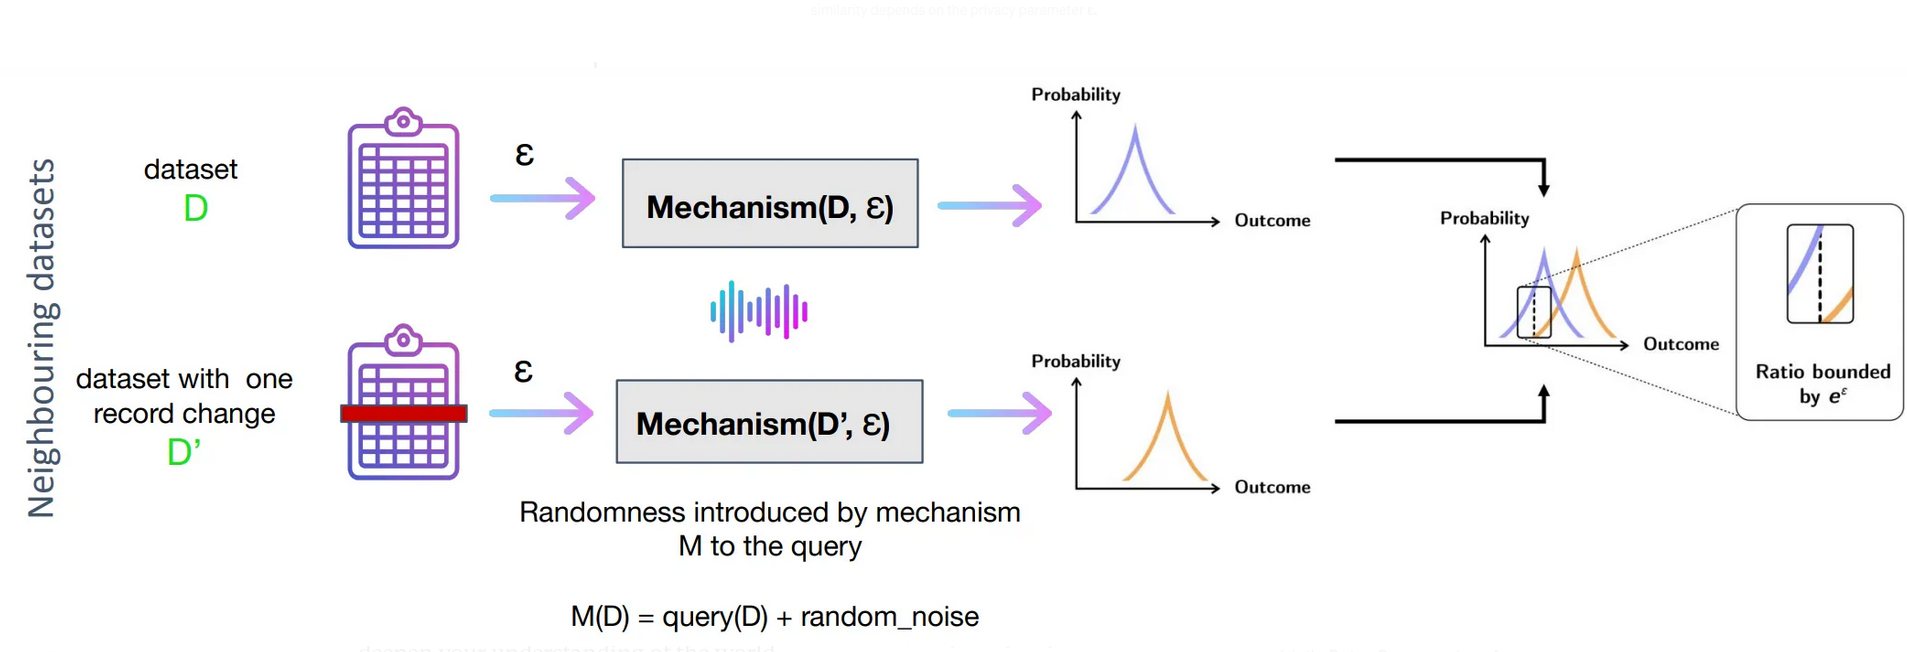
\includegraphics[scale=0.27]{dp_illustr.png}
        \caption{Illustration of DP\footnote{taken from: https://medium.com/dsaid-govtech/protecting-your-data-privacy-with-differential-privacy-an-introduction-abee1d7fcb63}}
        \label{fig:enter-label}
    \end{figure}

\end{frame}


\begin{frame}[fragile]
    \begin{tcblisting}{listing engine=minted,minted style=native,
        minted language=python,enhanced,
        colback=terminalColor,colframe=terminalColor,listing only, 
        image comment = {scale=0.25}{str.png},
        listing and comment,
        title=\tikz{
            \node[circle,fill=Button1,inner sep=3pt] (c) at (0,0){};
            \node[circle,fill=Button2,inner sep=3pt] (c) at (0.5,0){};
            \node[circle,fill=Button3,inner sep=3pt] (c) at (1,0){};
        }~~~~~~Terminal}
    \end{tcblisting}
\end{frame}

\begin{frame}[fragile]
    \frametitle{asd}

    \VerbatimInput[fontsize=\tiny]{../images/structure.txt}
   

\end{frame}